%\section{Calibration Hardware Overview}
%\label{sec:sp-calib-ov}


%%%%%%%%%%%%%%%%%%%%%%%%%%%%
%\fixme{SG:A paragraph length preamble 0 goes before Introduction as suggested by Tim; SG to edit in}

%\subsection{DUNE Calibration Strategy}
\label{sec:sp-calib-ov-intro}

%\fixme{(from Nora) I must point out that the headings in this document are problematic. They go to five levels, in some places (see page 7 on the PDF) with no text until the fifth level heading. This is extremely troubling. Generally, no heading should appear without at least transitional text following it, and here we have three headings with nothing, no content, no transitions, no indications of anything. This will not do. This is especially troublesome later in the chapter when bold is used to designate sections without using headings at all (see page 8 of the PDF). I strongly advise cutting the levels of heading down to three and making sure that text follows each heading. Major headings could use introductory text for that section/chapter while most subheadings should have content following. If you look, you will note that you already have text that can be used for those purposes. For instance, Section 1.1.1 is an introduction to the entire chapter. Some portions of this introduction appear to go with Section 1.1, the overview of the first part. One way to handle this is to put all the headings into a separate file and find the information that goes with the headings. You can then copy and paste the text to the appropriate section with the appropriate heading. If the heading has no text, that heading would be eliminated or text would be provided. This gives you a visual of how the paper fits together. One final note: too many headings cause confusion. (Too few headings also cause confusion.)}

A detailed understanding of the overall detector response is essential for DUNE physics goals. The precision with which each calibration parameter must be measured is set by the requirements on the %JM
systematic uncertainties for the \dword{lbl}, low-energy (\dword{snb}), and other physics programs at \dword{dune}. The calibration 
program 
%plan %JM;
must provide measurements at the few-percent-or-better 
%few-percent %JM; SG: this was a language edit from editors
level stably across an enormous volume and over a long period of time, and provide sufficient redundancy. The Physics volume of the \dword{tdr} provides a detailed description of the calibration strategy for the \dword{dune} \dword{fd}; here, we provide a brief summary.

The current calibration strategy for \dword{dune} uses existing sources of particles, external measurements, and dedicated external calibration hardware systems. Existing calibration sources for \dword{dune} include beam or atmospheric neutrino-induced samples, cosmic rays, argon isotopes, and instrumentation devices such as \lar purity and temperature monitors. Dedicated calibration hardware systems consist of laser, and neutron source deployment systems.  External measurements by \dword{protodune} and SBN experiments  will validate techniques, tools and the design of systems applicable to the \dword{dune} calibration program. These sources and systems provide measurements of the detector response model parameters, or provide tests of the response model itself. Calibration measurements can also provide corrections to data, data-driven efficiencies, systematics and particle responses.

%Chapter~4 of the Physics volume of the \dword{tdr} provides a more detailed description of the calibration strategy for the \dword{dune} \dword{fd}. 
%using existing sources of particles (e.g., cosmic ray muons), external measurements (e.g., \dword{protodune}), monitors (e.g., purity monitors), and dedicated calibration hardware systems. 

This chapter focuses on describing the dedicated calibration hardware systems to be deployed for the \dword{dune} \dword{spmod} that provide necessary information beyond the reach of external measurements and existing sources and monitors. These include an ionization laser system, a photoelectron laser system, and a \dlong{pns} system. The possibility of deploying a radioactive source system is also currently being explored. The responsibility of the calibration hardware systems fall under the joint \dword{sp} and \dword{dp} calibration consortium which was formed in November 2018.

%This chapter describes the design of the dedicated calibration systems to be deployed for the DUNE \spmod.  As discussed in the Physics TDR\fixme{proper reference}, the calibration strategy includes external measurements (e.g. ProtoDUNE), monitors (e.g. purity, thermal), existing sources of particles (e.g. muons from cosmic rays), and dedicated external calibration hardware systems.  This chapter discusses the calibration hardware systems. Monitoring systems are discussed in other chapters: CISC (purity, thermal monitors, slow control), PDS (LED stability system\fixme{proper name is?}), and CE (charge injection system). The physics TDR discusses the use of existing sources of particles, and external measurements. 

Once the far detector is filled and at the desired high voltage, it immediately becomes live for \dword{snb} and proton decay signals (beam and atmospheric neutrino physics will require a few years of data accumulation) at which point it is critical for %for %JM
early calibration to track %to track %JM
the space-time dependence of the detector. Dedicated early calibration runs using calibration hardware systems will develop and tune calibration tools to beam data taking and correct for any space-time irregularities observed in the \dword{tpc}. Given the expected low rate of cosmic ray events at the underground location, calibration with cosmic rays is not possible over short time scales and will proceed from coarse-grained to fine-grained over the course of years, as statistics accumulate. 
The experiment will rely on calibration hardware systems, such as a laser system, for calibrations that require an independent probe with reduced or removed interdependencies, fine-grained measurements (both in space and time), and detector stability monitoring on the time scales required by physics. Calibration systems such as neutron source system will provide low-energy electromagnetic response at the precision required for low-energy \dword{snb} physics. 
Once the detector is running stably, dedicated calibration runs, ideally before, during and after each run period, will ensure that detector conditions have not significantly changed. As DUNE becomes systematics-limited, dedicated precision-calibration campaigns using the calibration hardware systems will become crucial for meeting the stringent physics requirements on energy scale reconstruction and detector resolution.

%Section~\ref{sec:sp-calib-ov-scope} describes the baseline calibration hardware designs. 
%and outlines alternative designs that may improve the physics capability and/or reduce overall cost. 
Section~\ref{sec:sp-calib-ov} describes the baseline calibration hardware designs. Section~\ref{sec:sp-calib-sys-las-ion} describes the baseline design for the ionization laser system that provides an independent, fine-grained measurement of the electric field throughout the detector, which is an essential parameter that affects the spatial and energy resolution of physics signals. The DUNE \dword{cdr}~\cite{Acciarri:2015uup} assumes that the \dword{fv} is known to the \SI{1}{\%} level. Through measurements of the spatial distortions and drift velocity map, the laser calibration system mainly helps define the detector \dword{fv} thus allowing for the correct prediction of the \dword{fd} spectra. The laser system also offers many secondary uses such as alignment checks, stability monitoring, and diagnosing detector performance issues. Alternative designs for the ionization laser system that may improve the physics capability and/or reduce overall cost are also under development and are described in Appendix~\ref{sec:sp-calib-laser-alter}.
Section~\ref{sec:sp-calib-sys-las-pe} describes the photoelectron laser system that can be used to rapidly diagnose electronics or \dword{tpc} response issues along with many other useful measurements such as integrated field across drift, drift velocity, and electronics gain. 

Section~\ref{sec:sp-calib-sys-pns} describes the baseline design for the \dword{pns} system, which provides a triggered, well defined, energy deposition from neutron capture in Ar detectable throughout the detector volume. Neutron capture is a critical component of signal processes for \dword{snb} and \dword{lbl} physics, enabling direct testing of the detector response spatially and temporally for the low-energy program and the efficiency of the detector in reconstructing the low-energy spectra. The proposed \dword{rsds}, 
%radioactive source system
which is in many ways complementary to the \dword{pns}
%pulsed neutron source 
system, can provide at known locations inside the detector a source of gamma rays in the same energy range of \dword{snb} and solar neutrino physics. But the \dword{rsds} is the only calibration system that could probe the detection capability for single isolated solar neutrino events and study how well radiological backgrounds can be suppressed. In contrast, the \dword{pns} is externally triggered and does not provide such a well-defined source location for gamma rays inside the detector, but on the other hand the \dword{pns} can probe the uniformity of the full detector. The \dword{rsds} could only scan the ends of the detector. The proposed complementary \dword{rsds} system is described in the Appendix~\ref{sec:sp-calib-sys-rsds}. 

The \dword{daq} requirements for calibration systems are described in Section~\ref{sec:sp-calib-daqreq}. For all the calibration hardware systems, the goal is deploy prototype designs and validate them at \dword{protodune} as part of the post long shutdown 2 (LS2) running  at CERN. The validation plan for calibration systems at \dword{protodune} and other experiments is described in Section~\ref{sec:sp-calib-val}. 
The schedule and milestones for calibration systems is discussed in Section~\ref{sec:sp-calib-sched}.

%The calibration consortium was formed in November 2018. Significant development plans exist, and their timeline is in Section~\ref{sec:sp-calib-sched}.
%A large part of the work done so far has been done within the Calibration Task Force; 

%%%%%%%%%%%%%%%%%%%%%%%%%%%%
\subsection{Scope}
\label{sec:sp-calib-ov-scope}
% KM outline
%% Scope is: baseline designs for Laser system and neutron system.
%% Alternative designs, including additional capabilities of the laser system, radioactive source are considered.

%%calibration review in May. "what's the scope? How many lasers we need? How many ports needed? Do we need crossing tracks? do we need to penetrate FC ? what does the HV consortium think about that?"

The scope of the calibration consortium includes a laser ionization system, a photoelectron laser system, a laser positioning system, and a \dlong{pns}
%pulsed neutron source 
system. In addition, the consortium is evaluating a \dlong{rsds}
%radioactive source system
. The calibration consortium is responsible for design through commissioning in the \dword{sp} module for these calibration devices and their associated feedthroughs. Validating the designs of calibration systems at \dword{protodune} (and other experiments as relevant) is also included under the scope of the consortium. Figure~\ref{fig:calib_scope_chart} shows the subsystems included under the calibration consortium. 

Chapters 3, 4, 5, and 8 describe other hardware essential for calibration such as \dword{ce} external charge injection systems, \dword{hv} monitoring devices, \dword{pds},
stability monitoring system, and cryogenic instrumentation and detector monitoring devices. The scope of these systems are described by their respective consortia, and the calibration consortium has substantial interfaces with these consortia. 

The use of other calibration sources such as external measurements and existing sources of particles (e.g., muons, pions) is discussed in the physics volume of the \dword{tdr}. The calibration task force is pursuing the effects of calibration on physics and related studies, and the consortium works closely with the task force to make physics connections. Calibrations also require simulations (e.g. \efield) to identify desirable locations for calibration devices in the cryostat, away from regions of high \efield, so that their presence does not induce large field distortions. 
%Calibration has additional activities outside the scope of the consortium that require coordination with other groups. This is discussed in Section~\ref{sec:sp-calib-intfc}. 
The design of the calibration systems and understanding the related physics requires coordination with other consortia and groups. This is discussed in Section~\ref{sec:sp-calib-intfc}.
%, which also includes necessary tools (e.g., physics simulations) developed in conjunction with the physics groups and calibration task force.

%\fixme{Please use dunefigures! Here's a template (the label should be fig:filename):}

%\begin{dunefigure}[short caption]{label}
%{long caption}
%\includegraphics[width=0.8\textwidth]{filename}
%\end{dunefigure}

%\begin{figure}[tbp]
%\centering
%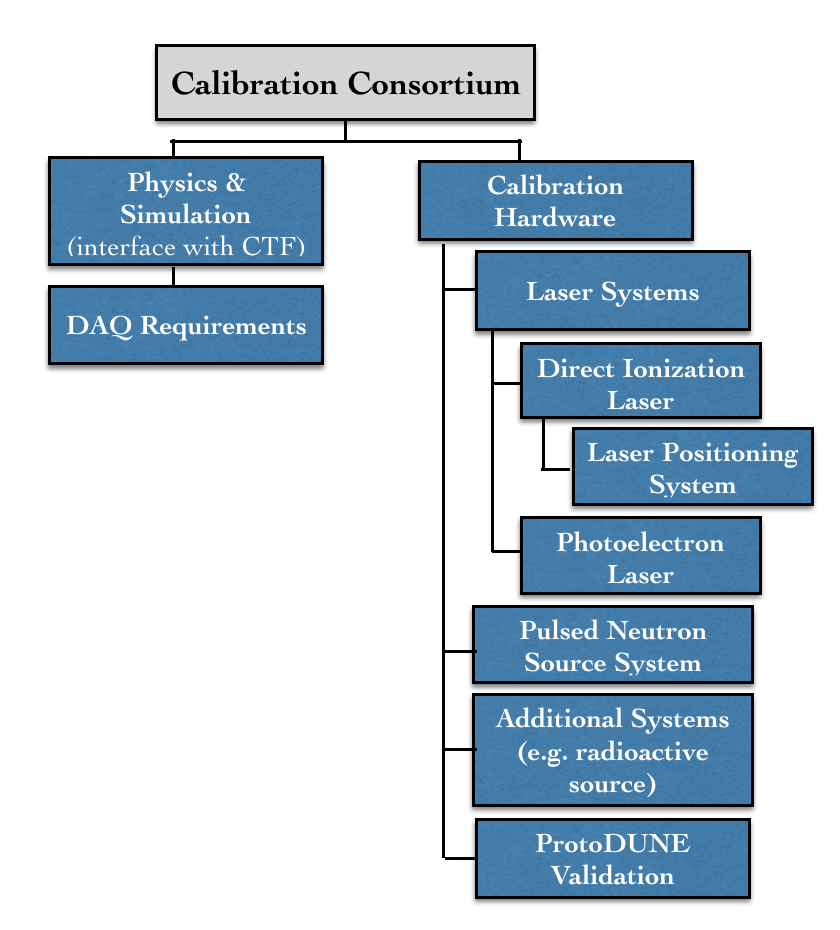
\includegraphics[height=4.0in]{graphics/calib_scope_chart.png}
%\caption{Calibration consortium subsystem chart.}
%\label{fig:scope_chart}
%\end{figure}

\begin{dunefigure}[Calibration consortium subsystem chart]{fig:calib_scope_chart}
{Calibration consortium subsystem chart.}
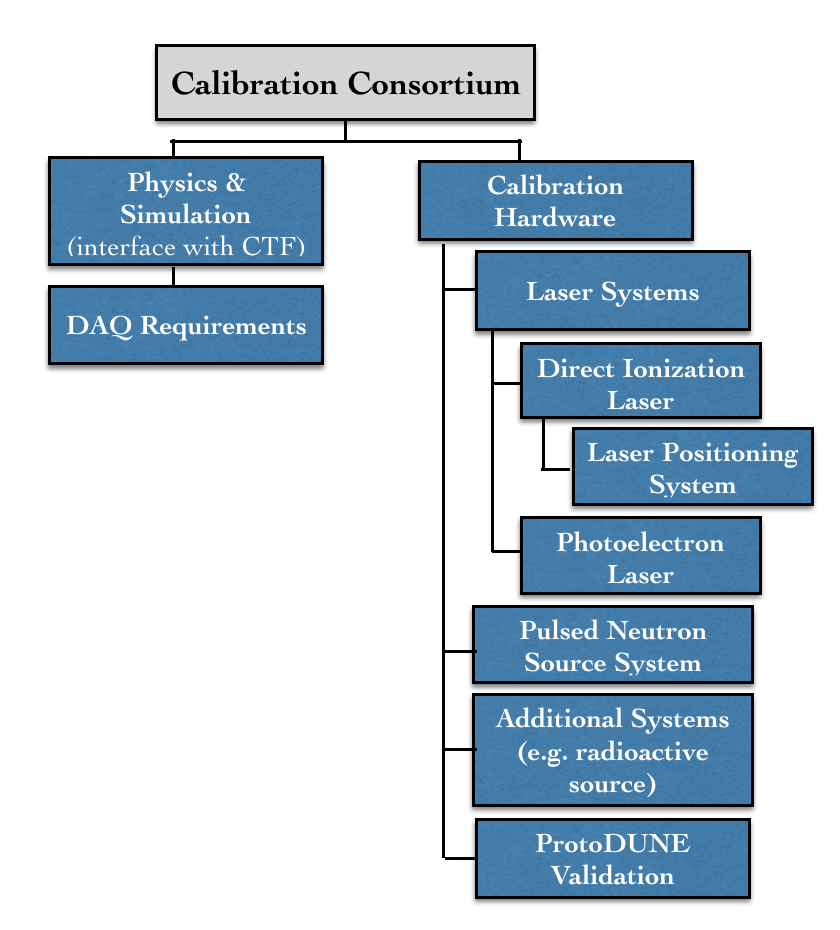
\includegraphics[height=4.0in]{graphics/calib_scope_chart.png}
\end{dunefigure}

%%%%%%%%%%%%%%%%%%%%%%%%%%%%
%\subsection{Requirements}
%\label{sec:sp-calib-ov-req}

%\input{vol-sp/ch-sp-calib-requirements}


%%%%%%%%%%%%%%%%%%%%%%%%%%%%
\subsection{Design Considerations and Requirements}
\label{sec:sp-calib-ov-consid}
%\fixme{SG, KM: Done; JM please check. }
%To-DO: Need more information on requirements from neutron source and RA source, once we have it, we can update the text/table as needed.}

Some common design considerations for calibration devices include stability, reliability, and longevity, so calibration systems can be operated for the lifetime of the experiment (\dunelifetime). Such longevity is uncommon for any device, so the overall design permits replacing devices where possible. The systems must also adhere to relevant global requirements of the \dword{dune} detector. Table~\ref{tab:specs:SP-CALIB} shows the top-level overall requirements for calibration subsystems. For example, \dword{dune} requires the \efield  on any instrumentation devices inside the cryostat to be less than 30 kV/cm to minimize the risk of dielectric breakdown in \lar. Another consideration important for reconstructing events is the maximum noise level the readout electronics can tolerate from calibration devices. \dword{pdsp} is evaluating this. 

 For the laser system, the energy and position reconstruction requirements for physics measurements lead to requirements for the necessary precision in measuring the laser \efield as well as its spatial coverage and granularity. The laser \efield measurement precision must be about \SI{1}{\%} so that the effect on the collected charge is well below \SI{1}{\%}. This is also motivated by consistency with the high level \dword{dune} specification of \SI{1}{\%} on field uniformity throughout the volume for component alignment and the \hv system. For laser coverage, to keep the \efield measurement at the $\sim$\SI{1}{\%} level, we are aiming for a coverage of \SI{75}{\%} or more of the total \dword{fv}. The requirement on granularity for the laser is estimated based on the \dword{fv} uncertainty requirements (\SI{1}{\%}) and corresponding uncertainty requirements (\SI{1.5}{\cm}) in each coordinate. A voxel size of \num{30}$\times$\num{30}$\times$\SI{30}{\cubic\cm} should be sufficient to satisfy the \dword{fv} uncertainty requirements. 

The laser beam position must also meet the level of reconstruction requirement in each coordinate, approximately \SI{5}{\milli\m} over \num{5} to \SI{10}{\m}, where the latter is the distance between two consecutive laser ports in the beam direction. This results in a stringent requirement of \ang{0.03} (or \SI{0.5}{\mrad}). The data volume for the ionization laser system must be at least \num{90}~TB/year/\SI{10}{\kt}, assuming \num{800}k laser pulses, \num{10}$\times$\num{10}$\times$\SI{10}{\cubic\cm} voxel sizes, a \SI{100}{\micro\s} zero suppression window, and one dedicated calibration campaign per year.

For the \dword{pns} system, the system must provide a sufficient neutron event rate to make spatially separated precision measurements across the detector of a comparable size to the voxels probed by the laser (\num{30}$\times$\num{30}$\times$\SI{30}{\cubic\cm}) for most regions of the detector (\SI{75}{\%}). 
% 1st draft
%For the supernova program, measurements from the \dword{pns} \fixme{This abbreviation is in neither glossary.} should demonstrate 1\% energy scale, 5\% energy resolution, and 0.5 MeV detection threshold, so each voxel should have sufficient neutron event rate to achieve this. %\todo{KM: Improve or remind connection to SN program? even though it's comparable? SG: maybe for 2nd draft?}
%rewritten for 2nd draft
For the supernova program, the sensitivity to distortions of the neutrino energy spectrum is dependent on the uncertainties in the detection threshold and the reconstructed energy scale and resolution. Studies discussed in the physics \dword{tdr} present target ranges for the uncertainties in these parameters as a function of energy. The measurements with the \dword{pns} aim to provide response corrections and performance estimates such that those uncertainty targets are met throughout the whole volume, and so that each voxel should have a sufficient neutron event rate (percent level statistical uncertainty).

%\fixme{Insert correct reference to physics TDR ch7}
%\fixme{Put PNS in glossary and use that.}


In terms of data volume requirements, the \dword{pns} system requires about \num{84}~TB/year/\SI{10}{\kt} assuming \num{e6} neutrons/pulse, \num{1000} neutron captures/\si{\cubic\m}
%m$^{3}$ 
and \num{1300} observed neutron captures per pulse, and six calibration runs per year. 



Table~\ref{tab:fdgen-calib-all-reqs} shows the full set of requirements related to all calibration subsystems. More details on each of the requirements can be found under corresponding consortia.   
\todo{SP-CALIB-3 is coming out weird in table 1.1, needs to be fixed.}

%\fixme{Can the second part of this title be put in a footnote to Table 1.1? SG: we would prefer to leave it here}


%% This file is generated, any edits may be lost.

\begin{longtable}{p{0.14\textwidth}p{0.13\textwidth}p{0.18\textwidth}p{0.22\textwidth}p{0.20\textwidth}}
\caption{Specifications for SP-CALIB \fixmehl{ref \texttt{tab:spec:SP-CALIB}}} \\
  \rowcolor{dunesky}
       Label & Description  & Specification \newline (Goal) & Rationale & Validation \\  \colhline

   \newtag{SP-CALIB-1}{ spec:efield-calib-precision }  & Ionization laser electric field measurement precision  &  \SI{1}{\%} \newline ( $<$\SI{1}{\%} ) &  Electric field affects energy and position measurements. &  ProtoDUNE and external experiments. \\ \colhline
     % 1
   \newtag{SP-CALIB-2}{ spec:efield-calib-coverage }  & Ionization laser \efield measurement coverage  &  $>\,\SI{75}{\%}$ \newline ( \SI{100}{\%} ) &  Allowable size of the uncovered detector regions is set by the highest reasonably expected field distortions, 4%. &  ProtoDUNE \\ \colhline
     % 2
   \newtag{SP-CALIB-3}{ spec:efield-calib-granularity }  & Ionization laser \efield measurement  granularity  &  $<\,\SI{30\times30\times30}{\centi\meter}$ \newline ( $<\,\SI{10\times10\times10}{\centi\meter}$ ) &  Minimum measurable region is set by the maximum expected distortion and position reconstruction requirements. &  ProtoDUNE \\ \colhline
     % 3
   \newtag{SP-CALIB-4}{ spec:laser-position-precision }  & Laser beam position precision  &  $~\SI{0.5}{\milli\radian}$ \newline ($<\SI{0.5}{\milli\radian}$) &  The necessary spatial precision does not need to be smaller than the APA wire gap. &  ProtoDUNE \\ \colhline
     % 4
   \newtag{SP-CALIB-5}{ spec:neutron-source-coverage }  & Neutron source coverage  &  $>$\SI{75}{\%} \newline ( \SI{100}{\%} ) &  The coverage of the pulsed neutron system depends on the energy resolution requirements at low energy. &  Simulations \\ \colhline
     % 5
   \newtag{SP-CALIB-6}{ spec:data-volume-laser }  & Ionization laser data volume per year (per 10 kt)  &  $>\SI{184}{TB/yr/10 kt}$ \newline ($>\SI{368}{TB/yr/10 kt}$) &  The laser data volume must allow the needed coverage and granularity. &  ProtoDUNE and simulations \\ \colhline
     % 6
   \newtag{SP-CALIB-7}{ spec:data-volume-pns }  & Neutron source DAQ rate per year (per 10 kton)  &  $>$\SI{84}{TB/yr/10 kton} \newline ( $>$\SI{168}{TB/yr/10 kton} ) &  The coverage of the pulsed neutron system depends on the energy resolution requirements at low energy. &  Simulations \\ \colhline
     % 7


\label{tab:specs:just:SP-CALIB}
\end{longtable}

% This file is generated, any edits may be lost.

\begin{longtable}{p{0.14\textwidth}p{0.13\textwidth}p{0.18\textwidth}p{0.22\textwidth}p{0.20\textwidth}}
\caption{Specifications for SP-CALIB \fixmehl{ref \texttt{tab:spec:SP-CALIB}}} \\
  \rowcolor{dunesky}
       Label & Description  & Specification \newline (Goal) & Rationale & Validation \\  \colhline

   \newtag{SP-FD-1}{ spec:min-drift-field }  & Minimum drift field  &  $>$\,\SI{250}{ V/cm} \newline ( $>\,\SI{500}{ V/cm}$ ) &  Lessens impacts of $e^-$-Ar recombination, $e^-$ lifetime, $e^-$ diffusion and space charge. &  ProtoDUNE \\ \colhline
    
   
  \newtag{SP-FD-2}{ spec:system-noise }  & System noise  &  $<\,\SI{1000}\,e^-$ &  Provides $>$5:1 S/N on induction planes for  pattern recognition and two-track separation. &  ProtoDUNE and simulation \\ \colhline
    
   
  \newtag{SP-FD-3}{ spec:light-yield }  & Light yield  &  $>\,\SI{20}{PE/MeV}$ (avg), $>\,\SI{0.5}{PE/MeV}$ (min) &  Gives PDS energy resolution comparable that of the TPC for 5-7 MeV SN $\nu$s, and allows tagging of $>\,\SI{99}{\%}$ of nucleon decay backgrounds with light at all points in detector. &  Supernova and nucleon decay events in the FD with full simulation and reconstruction. \\ \colhline
    
    \\ \rowcolor{dunesky} \newtag{SP-FD-4}{ spec:time-resolution-pds } & Name: Time resolution \\
    Description & The time resolution of the photon detection system shall be less than 1 microsecond in order to assign a unique event time.   \\  \colhline
    Specification (Goal) &  $<\,\SI{1}{\micro\second}$  ( $<\,\SI{100}{\nano\second}$ ) \\   \colhline
    Rationale &   Enables \SI{1}{mm} position resolution for \SI{10}{MeV} SNB candidate events for instantaneous rate $<\,\SI{1}{m^{-3}ms^{-1}}$.  \\ \colhline
    Validation &   \\
   \colhline

   \newtag{SP-FD-5}{ spec:lar-purity }  & Liquid argon purity  &  $<$\,\SI{100}{ppt} \newline ($<\,\SI{30}{ppt}$) &  Provides $>$5:1 S/N on induction planes for  pattern recognition and two-track separation. &  Purity monitors and cosmic ray tracks \\ \colhline
    
    \\ \rowcolor{dunesky} \newtag{SP-FD-7}{ spec:misalignment-field-uniformity } & Name: Drift field uniformity due to component alignment \\
    Description & Misalignments of the various TPC components shall not introduce drift-field nonuniformities beyond those specified in the HVS requirements.   \\  \colhline
    Specification &  $<\,1\,$\% throughout volume \\   \colhline
    Rationale &   Maintains APA, CPA,  FC orientation and shape.  \\ \colhline
    Validation & ProtoDUNE  \\
   \colhline

    
   
  \newtag{SP-FD-9}{ spec:apa-wire-spacing }  & APA wire spacing  &  \SI{4.669}{mm} for U,V; \SI{4.790}{mm} for X,G &  Enables 100\% efficient MIP detection, \SI{1.5}{cm} $yz$ vertex resolution. &  Simulation \\ \colhline
    
    \\ \rowcolor{dunesky} \newtag{SP-FD-11}{ spec:hvs-field-uniformity } & Name: Drift field uniformity due to HVS \\
    Description & Design of TPC cathode and FC components shall ensure uniform field.  Production tolerances shall be set so as to maintain flatness of component surfaces and, by extension, the shape of the drift field volume.   \\  \colhline
    Specification &  $<\,\SI{1}{\%}$ throughout volume \\   \colhline
    Rationale &   High reconstruction efficiency.  \\ \colhline
    Validation & ProtoDUNE and simulation  \\
   \colhline

    
   \newtag{SP-FD-13}{ spec:fe-peak-time }  & Front-end peaking time  &  \SI{1}{\micro\second} \newline ( Adjustable so as to see saturation in less than \SI{10}{\%} of beam-produced events ) &  Vertex resolution; optimized for \SI{5}{mm} wire spacing. &  ProtoDUNE and simulation \\ \colhline
    
   
  \newtag{SP-FD-16}{ spec:det-dead-time }  & Detector dead time  &  $<\,\SI{0.5}{\%}$ &  Meet physics goals in timely fashion. &  ProtoDUNE \\ \colhline
    
   
  \newtag{SP-FD-22}{ spec:data-rate-to-tape }  & Data rate to tape  &  $<\,\SI{30}{PB/year}$ &  Cost.  Bandwidth. &  ProtoDUNE \\ \colhline
    
   
  \newtag{SP-FD-23}{ spec:sn-trigger }  & Supernova trigger  &  $>\,\SI{90}{\%}$ efficiency for SNB within \SI{100}{kpc} &  $>\,$90\% efficiency for SNB within 100 kpc &  Simulation and bench tests \\ \colhline
    
    \\ \rowcolor{dunesky} \newtag{SP-FD-24}{ spec:local-e-fields } & Name: Local electric fields \\
    Description & The integrated detector design shall minimize potential pathways for HV discharges.   \\  \colhline
    Specification &  $<\,\SI{30}{kV/cm}$ \\   \colhline
    Rationale &   Maximize live time; maintain high S/N.  \\ \colhline
    Validation & ProtoDUNE  \\
   \colhline

   
  \newtag{SP-FD-25}{ spec:non-fe-noise }  & Non-FE noise contributions  &  $<<\,\SI{1000}{enc} $ &  High S/N for high reconstruction efficiency. &  Engineering calculation and ProtoDUNE \\ \colhline
    
    \\ \rowcolor{dunesky} \newtag{SP-FD-26}{ spec:lar-impurity-contrib } & Name: LAr impurity contributions from components \\
    Description & Contributions to LAr contamination from detector components, through outgassing or other processes, shall remain << 30 ppt so as to avoid significantly increasing the nominal level of contamination.   \\  \colhline
    Specification &  $<<\,\SI{30}{ppt} $ \\   \colhline
    Rationale &   Maintain HV operating range for high live time fraction.  \\ \colhline
    Validation & ProtoDUNE  \\
   \colhline

    \\ \rowcolor{dunesky} \newtag{SP-FD-27}{ spec:radiopurity } & Name: Introduced radioactivity \\
    Description & Introduced radioactivity shall be less than that from 39Ar.   \\  \colhline
    Specification &  less than that from $^{39}$Ar \\   \colhline
    Rationale &   Maintain low radiological backgrounds for SNB searches.  \\ \colhline
    Validation & ProtoDUNE and assays during construction  \\
   \colhline


   \newtag{SP-CALIB-1}{ spec:efield-calib-precision }  & Ionization laser electric field measurement precision  &  \SI{1}{\%} \newline ( $<$\SI{1}{\%} ) &  Electric field affects energy and position measurements. &  ProtoDUNE and external experiments. \\ \colhline
    
   \newtag{SP-CALIB-2}{ spec:efield-calib-coverage }  & Ionization laser \efield measurement coverage  &  $>\,\SI{75}{\%}$ \newline ( \SI{100}{\%} ) &  Allowable size of the uncovered detector regions is set by the highest reasonably expected field distortions, 4%. &  ProtoDUNE \\ \colhline
    
   \newtag{SP-CALIB-3}{ spec:efield-calib-granularity }  & Ionization laser \efield measurement  granularity  &  $<\,\SI{30\times30\times30}{\centi\meter}$ \newline ( $<\,\SI{10\times10\times10}{\centi\meter}$ ) &  Minimum measurable region is set by the maximum expected distortion and position reconstruction requirements. &  ProtoDUNE \\ \colhline
    
   \newtag{SP-CALIB-4}{ spec:laser-position-precision }  & Laser beam position precision  &  $~\SI{0.5}{\milli\radian}$ \newline ($<\SI{0.5}{\milli\radian}$) &  The necessary spatial precision does not need to be smaller than the APA wire gap. &  ProtoDUNE \\ \colhline
    
   \newtag{SP-CALIB-5}{ spec:neutron-source-coverage }  & Neutron source coverage  &  $>$\SI{75}{\%} \newline ( \SI{100}{\%} ) &  The coverage of the pulsed neutron system depends on the energy resolution requirements at low energy. &  Simulations \\ \colhline
    
   \newtag{SP-CALIB-6}{ spec:data-volume-laser }  & Ionization laser data volume per year (per 10 kt)  &  $>\SI{184}{TB/yr/10 kt}$ \newline ($>\SI{368}{TB/yr/10 kt}$) &  The laser data volume must allow the needed coverage and granularity. &  ProtoDUNE and simulations \\ \colhline
    
   \newtag{SP-CALIB-7}{ spec:data-volume-pns }  & Neutron source DAQ rate per year (per 10 kton)  &  $>$\SI{84}{TB/yr/10 kton} \newline ( $>$\SI{168}{TB/yr/10 kton} ) &  The coverage of the pulsed neutron system depends on the energy resolution requirements at low energy. &  Simulations \\ \colhline
    
   
  \newtag{SP-CALIB-8}{ spec:rate-gammas-source }  & Rate of 9 MeV capture gamma events in the proposed radioactive source  &  $<\,\SI{1}{\kilo\hertz}$ &  The source rate must be such that there is no more than one event per drift time. &  Lab tests \\ \colhline
    


\label{tab:specs:SP-CALIB}
\end{longtable}

\begin{comment}
%comment the old "hand-made" latex table

\begin{dunetable}
[Top-level specifications for calibration subsystems]
{p{0.45\linewidth}p{0.25\linewidth}p{0.25\linewidth}}
{tab:fdgen-calib-toplevel-reqs} 
{List of Top-Level Specifications for the Calibration Subsystems. Global DUNE requirements are listed in bold.}   Quantity/Parameter	& Specification	& Goal		 \\ \toprowrule      
{\bf Noise from calibration devices}	 & $\ll$ 1000 enc   & \\ \colhline    
{\bf Max. \efield near calibration devices} & < 30 kV/cm & <15 kV/cm \\ \colhline     
Ionization Laser \efield measurement precision & 1\% & <1\% \\ \colhline
Ionization Laser \efield measurement coverage & > 75\% & 100\% \\ \colhline
Ionization Laser \efield measurement granularity & < \num{30}x\num{30}x\num{30}~cm & \num{10}x\num{10}x\num{10}~cm \\ \colhline
Laser beam position precision & 0.5 mrad & 0.5 mrad \\ \colhline
Neutron source coverage & > 75\% & 100\% \\ \colhline % neutron source
Ionization laser DAQ rate (per 10 kton) & 90~TB/year & 185~TB/year\\ \colhline
Neutron source DAQ rate (per 10~kton) & 84~TB/year & 168~TB/year\\ \colhline
Rate of 9~MeV capture $\gamma$-events inside the proposed radioactive source & < 1~kHz & \\ \colhline 
\end{dunetable}
\end{comment}

\begin{dunetable}
[Full specifications for calibration subsystems]
{p{0.45\linewidth}p{0.25\linewidth}p{0.25\linewidth}}
{tab:fdgen-calib-all-reqs}
{Full list of Specifications for the Calibration Subsystems.}   
Quantity/Parameter	& Specification	& Goal		 \\ \toprowrule      

Noise from calibration devices	 & $\ll$ 1000 enc   & \\ \colhline    Max. \efield near calibration devices & < 30 kV/cm & <15 kV/cm \\ \colhline                     

\textbf{Direct Ionization Laser System} &    &   \\ \colhline   
\efield measurement precision & 1\% & <1\% \\ \colhline
\efield measurement coverage & > 75\% & 100\% \\ \colhline
\efield measurement granularity & < \num{30}x\num{30}x\num{30}~cm & \num{10}x\num{10}x\num{10}~cm \\ \colhline
Top field cage penetrations (alternative design) & to achieve desired laser coverage & \\ \colhline
DAQ rate per 10~kton & 90 TB/year & 185 TB/year \\ \colhline
Longevity	& \dunelifetime			& > \dunelifetime   \\ \colhline        
%Stability & Match precision requirement at all places/times	&  \\ \colhline  Reliability	& Measurements as needed & Measurements as needed \\ \colhline 
\textbf{Laser Positioning System} & & \\ \colhline                      
Laser beam position precision & 0.5~mrad & 0.5~mrad \\ \colhline
Longevity	& \dunelifetime			& > \dunelifetime   \\ \colhline        
%Stability & Match precision requirement at all places/times	&  \\ \colhline  Reliability	& Measurements as needed & Measurements as needed \\ \colhline    
\textbf{Photoelectron Laser System}	   &   &  \\ \colhline            
Longevity	& \dunelifetime			& > \dunelifetime   \\ \colhline        
%Stability & Match precision requirement at all places/times	&  \\ \colhline  Reliability	& Measurements as needed & Measurements as needed \\ \colhline

\textbf{Pulsed Neutron Source System}	   &   &  \\ \colhline        
Coverage & > 75\% & 100\% \\ \colhline
DAQ rate per 10~kton & 84~TB/year & 168~TB/year \\ \colhline 
Longevity	& 3 years			& \dunelifetime   \\ \colhline        
%Stability & Match precision requirement at all places/times	&  \\ 
%\colhline  Reliability	& Measurements as needed & Measurements as needed \\ \colhline

%\textbf{Proposed Radioactive Source System}	   &   &  \\ \colhline  
%Distance of the source from the field cage & 30 cm & \\ \colhline
%Rate of 9~MeV capture $\gamma$-events inside the source & < 1kHz & \\ \colhline 
%Data volume per 10~kton & 50~TB/year & 100~TB/year \\ \colhline 
%Longevity	& \dunelifetime			& > \dunelifetime   \\ \colhline    
%Stability & Match precision requirement at all places/times	&  \\ \colhline  Reliability	& Measurements as needed & Measurements as needed \\ \colhline

\end{dunetable}







\subsection{Cryostat Configuration for Calibration}
\label{sec:calib-ports}
Figure~\ref{fig:FTmap} shows the current cryostat design for the %DUNE SP FD 
\spmod with penetrations for various sub-systems. The penetrations dedicated for calibrations are the highlighted black circles. The ports on far east and far west are outside the \dword{fc}. The current plan is to use these penetrations for several different purposes. For example, the penetrations on the far east and west will be used both by laser and radioactive source systems (if deployed). In addition to these dedicated ports, the \dword{dss} and cryogenic ports (orange and blue dots in Figure~\ref{fig:FTmap}) will also be used as needed to route cables for calibration systems (e.g., the \dword{sp} \dword{pds}). \dword{dss} and cryogenic ports can be accommodated with feedthroughs with a CF63 side flange for this purpose.   

%\begin{figure}[tbp]
%\centering
%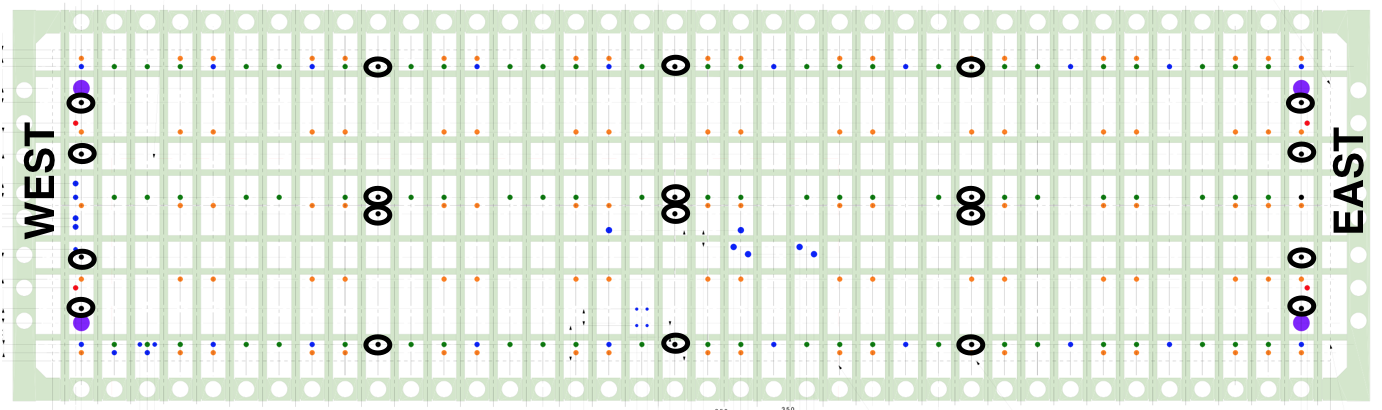
\includegraphics[height=2.0in]{FTmap.png}
%\caption{Top view of the \spmod %DUNE SP FD 
%cryostat showing various penetrations. Circles highlighted in black are multi-purpose calibration penetrations. The green dots are \dword{tpc} signal cable penetrations. The blue ports are cryogenic ports. The orange ports are \dword{dss} penetrations. The larger purple ports at the four corners of the cryostat are human access ports.}
%\label{fig:ftmap}
%\end{figure}

\begin{dunefigure}[Cryostat penetration map with calibration ports]{fig:FTmap}
{Top view of the \spmod %DUNE SP FD 
cryostat showing various penetrations. Circles highlighted in black are multi-purpose calibration penetrations. The green dots are \dword{tpc} signal cable penetrations. The blue ports are cryogenic ports. The orange ports are \dword{dss} penetrations. The larger purple ports at the four corners of the cryostat are human access ports.}
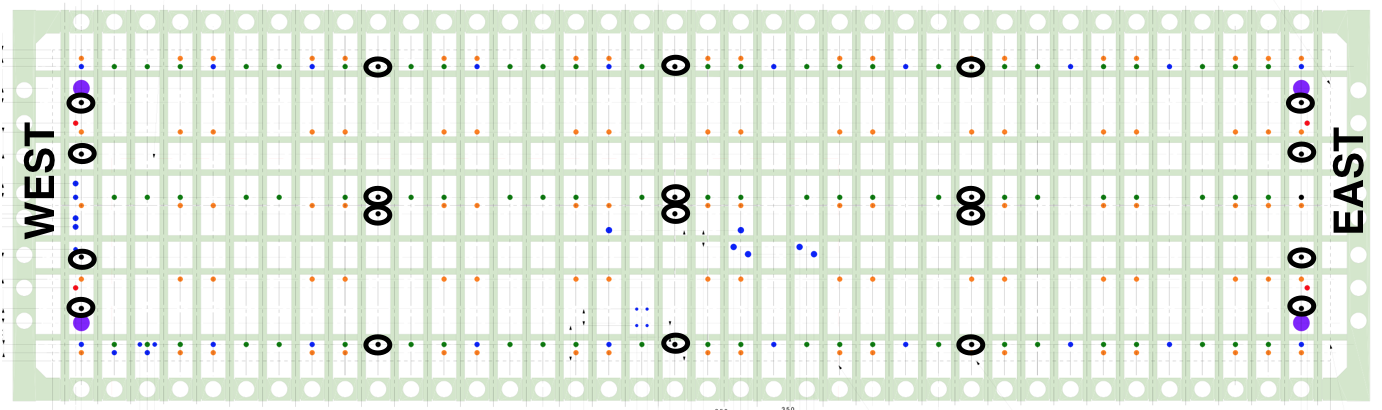
\includegraphics[height=2.0in]{FTmap.png}
\end{dunefigure}





The placement of these penetrations is largely driven by requirements for the ionization track laser. %and radioactive source system. 
The ports that are %inwards 
towards the center of the cryostat are placed near the \dwords{apa} to minimize any risks due to the \dword{hv} discharge. For the far east and west ports, \dword{hv} is not an issue as they are located outside the \dword{fc} and the penetrations are located near mid-drift (location favorable to possible source deployment).
%to meet radioactive source requirements. 
%\fixme{The amendment above may need some work. I won't look at it until it's ready.}
Implementing the ionization track laser system as proposed in Section~\ref{sec:sp-calib-sys-las-ion} requires \num{20} feedthroughs at the four \dword{tpc} drift volumes; this arrangement allows lasers to be used for full volume calibration of the E field and associated diagnostics (e.g., \dword{hv}). 

The distance between any two consecutive feedthrough columns in Figure~\ref{fig:FTmap} should be approximately \SI{15}{\m}, which is reasonable because experience from the \microboone laser system shows that tracks will propagate over that detector's full \SI{10}{\m} length. Assuming that the effects of Rayleigh scattering and self-focusing (Kerr effect) do not limit the laser track length, this laser arrangement could illuminate the full volume with crossing track data.  Please note that at this time, the maximum usable track length is unknown, and it may be that the full \SI{60}{\m} \detmodule length could be covered by the laser system after optimization.


